Section \ref{section:ExperimentComparisonTimeLengths} revealed, that the 2h time length (from the 3h dataset) produced the most distinct and well defined clusters, according to the evaluation scores. The order of the other top performing time lengths was further assessed. By eliminating the winning column from figure \ref{figure:clusteringResults8} iteratively and comparing the resulting time lengths (see figure \ref{figure:clusterResultsPlaces} in appendix \ref{appendix:clusteringEvaluationResults}), the following order can be assumed: 2h (3h), 1h (1h), 1h (3h), 30 min (1h), 30 min (3h), and 15 min (1h). 1h (3h) out performs when compared directly to 30 min (1h). The direct comparison, for example, of 30 min (1h), 1h (1h), and 1h (3h) (figure \ref{figure:clusterResultsPlaces2} in appendix \ref{appendix:clusteringEvaluationResults}) however, results in 1h (3h) placing first, 1h (1h) placing second and 30 min (1h) placing third. When considering the highest number of evaluation score "wins" over different t-SNE and clustering results, the 30 min time delta (from the 1h dataset) came top, followed by the 1h time length and then the 2h time length (both from the 3h dataset) (see figure \ref{figure:clusteringResultsGraphTotal}). These final results show, that the exact placing of these time lengths is hard to determine, since it depends on how they were compared. However, 2h (3h), 1h (3h), 1h (1h), and 30 min (1h) proved to be the bester performers.
The 45 minute time delta in the 1 hour data files appeared to perform the lowest, with 0 wins. The fact that 45 never out performed the other time lengths shows consistency, despite the different results.
 


\begin{figure}
  \centering
  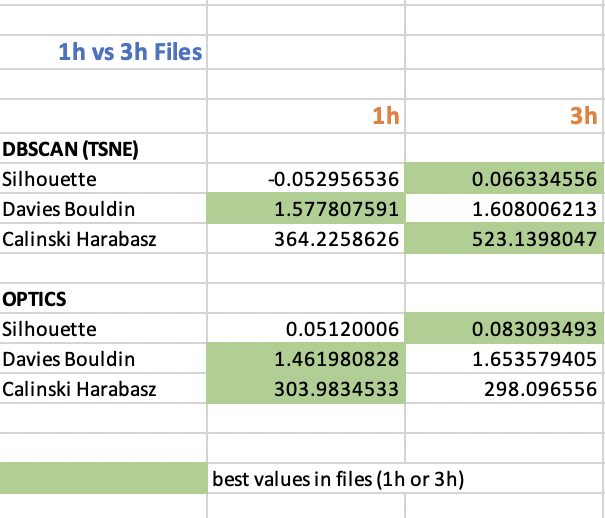
\includegraphics[width=0.5\textwidth]{./images/clusteringResults/clusteringResults7.png}
  \caption{Evaluation scores comparison from \textbf{averaged 1h and 3h dataset} runs of t-SNE and clustering.}
  \label{figure:clusteringResults7}
\end{figure}


The results from \textcite{AboutToEat2016Rahman} (as mentioned in section \ref{section:RelatedWork}) showed, that higher time lengths (e.g. 100 minutes) performed better than shorter ones. They deducted, that smaller window sizes were susceptible to noise and had a higher gap between precision (exactness) and recall (completeness). This discovery could also apply to the results of this experiment, considering that the 2h and 1h time lengths placed in the top three results.

To determine whether the 1 hour or 3 hour aggregation files led to better clusters, the average results of both time files are compared in figure \ref{figure:clusteringResults7}. Both the 1h and 3h datasets have the same number of wins. When scanning other comparisons of the evaluation scores (also the ones utilised for finding the t-SNE parameters), it is noticeable, that the 1h and 3h datasets either have the same number of wins, or the 3h dataset has more. This indicates that overall, the three hour aggregation files produce more superior clusters. Of the 36 number of wins across all time deltas (the 1h and 3h aggregation files combined), 14 of these were achieved by the 1h data file time lengths (38.9\%), the other 22 by the 3 hour dataset (61.1\%). A possible explanation, as to why the 3h dataset might have created better clusters, was that the cleaned dataset had more rows (as revealed in section \ref{section:chainShapedData}). The use of more data could have resulted in more similar rows and more improved clusters. Another aspect to consider, is that sensor data recorded for shorter time lengths might not be long enough to detect underlying stress patterns. There were also shorter intervals in between the recordings of the 3h dataset (1.5h instead of 2.5 for the 1h dataset). Therefore, less time was missed, where important patterns might have occurred.

Moreover, the higher the number of rows, the more robust the clusters could be towards potential outliers. As explained in section \ref{section:silhouetteCoefficient}, the Silhouette Score compares the within cluster distances to the distance of a neighbouring cluster. If many points are well placed within a cluster, an outlier will have little impact against the many short distances. However, if the cluster is not very dense and only contains a few "good" assigned data points, an outlier could have a larger impact on the result.

In order to provide Just-in-Time Intervention, the SmartEater app would need to predict upcoming stress. There are different types of stress. The Canadian Centre for Studies on Human Stress (CSHS) \footnote{\url{https://humanstress.ca/stress/understand-your-stress/acute-vs-chronic-stress/}} differentiate acute and chronic stress. Acute stress is caused by a particular event or setting, when something is new and feels out of control (e.g. presentations). Chronic stress is longer term and caused by repeated situations that cause stress. The data points would need to account for and recognise these different types of stress. For example, if stress is short, then a longer time delta will likely make it seem less relevant, compared to all the unstressed data. However, if it is long, a shorter time delta might miss it or only perceive a small part of it. This could be a reason why middle time lengths, such as 2h, 1h (3h data files) and 30 min (1h) created more distinct clusters, since they may have been more likely to recognise these differences. The fact that there was not one specific time length that always performed higher than the others shows, that a single time length may not be enough to be able to create clear clusters. Different time lengths might be needed to detect different patterns. Since the 3h data files appeared to perform better, this could point to the fact that stress requires a longer time period to predict. The 3h files also appear to have more, but smaller clusters. This variety could indicate, that more various types of stress were able to be found.

For future work, it might be beneficial to collect more data from users for a longer period of time. However, it would also be necessary to confirm that the clusters were created for stress levels and not for each user (since a user's behaviour could exhibit similarities). As implemented in this thesis, this could be observed by highlighting each user's results with a unique colour. It might also be beneficial to support the mathematical evaluations with hand drawn clusters found by test users in user studies. Especially since the scores are different each time t-SNE is computed, sometimes leading to different results. As mentioned in section \ref{section:TheoryDataMining} by \textcite{DataMiningAndPredictiveAnalytics}[9], data mining requires continuous human supervision for quality monitoring and evaluation.

